\documentclass[floatsintext,man]{apa6}

\usepackage{amssymb,amsmath}
\usepackage{ifxetex,ifluatex}
\usepackage{fixltx2e} % provides \textsubscript
\ifnum 0\ifxetex 1\fi\ifluatex 1\fi=0 % if pdftex
  \usepackage[T1]{fontenc}
  \usepackage[utf8]{inputenc}
\else % if luatex or xelatex
  \ifxetex
    \usepackage{mathspec}
    \usepackage{xltxtra,xunicode}
  \else
    \usepackage{fontspec}
  \fi
  \defaultfontfeatures{Mapping=tex-text,Scale=MatchLowercase}
  \newcommand{\euro}{€}
\fi
% use upquote if available, for straight quotes in verbatim environments
\IfFileExists{upquote.sty}{\usepackage{upquote}}{}
% use microtype if available
\IfFileExists{microtype.sty}{\usepackage{microtype}}{}

% Table formatting
\usepackage{longtable, booktabs}
\usepackage{lscape}
% \usepackage[counterclockwise]{rotating}   % Landscape page setup for large tables
\usepackage{multirow}		% Table styling
\usepackage{tabularx}		% Control Column width
\usepackage[flushleft]{threeparttable}	% Allows for three part tables with a specified notes section
\usepackage{threeparttablex}            % Lets threeparttable work with longtable

% Create new environments so endfloat can handle them
% \newenvironment{ltable}
%   {\begin{landscape}\begin{center}\begin{threeparttable}}
%   {\end{threeparttable}\end{center}\end{landscape}}

\newenvironment{lltable}
  {\begin{landscape}\begin{center}\begin{ThreePartTable}}
  {\end{ThreePartTable}\end{center}\end{landscape}}




% The following enables adjusting longtable caption width to table width
% Solution found at http://golatex.de/longtable-mit-caption-so-breit-wie-die-tabelle-t15767.html
\makeatletter
\newcommand\LastLTentrywidth{1em}
\newlength\longtablewidth
\setlength{\longtablewidth}{1in}
\newcommand\getlongtablewidth{%
 \begingroup
  \ifcsname LT@\roman{LT@tables}\endcsname
  \global\longtablewidth=0pt
  \renewcommand\LT@entry[2]{\global\advance\longtablewidth by ##2\relax\gdef\LastLTentrywidth{##2}}%
  \@nameuse{LT@\roman{LT@tables}}%
  \fi
\endgroup}


  \usepackage{graphicx}
  \makeatletter
  \def\maxwidth{\ifdim\Gin@nat@width>\linewidth\linewidth\else\Gin@nat@width\fi}
  \def\maxheight{\ifdim\Gin@nat@height>\textheight\textheight\else\Gin@nat@height\fi}
  \makeatother
  % Scale images if necessary, so that they will not overflow the page
  % margins by default, and it is still possible to overwrite the defaults
  % using explicit options in \includegraphics[width, height, ...]{}
  \setkeys{Gin}{width=\maxwidth,height=\maxheight,keepaspectratio}
\ifxetex
  \usepackage[setpagesize=false, % page size defined by xetex
              unicode=false, % unicode breaks when used with xetex
              xetex]{hyperref}
\else
  \usepackage[unicode=true]{hyperref}
\fi
\hypersetup{breaklinks=true,
            pdfauthor={},
            pdftitle={Mid Term Project Report : Predict 413},
            colorlinks=true,
            citecolor=blue,
            urlcolor=blue,
            linkcolor=black,
            pdfborder={0 0 0}}
\urlstyle{same}  % don't use monospace font for urls

\setlength{\parindent}{0pt}
%\setlength{\parskip}{0pt plus 0pt minus 0pt}

\setlength{\emergencystretch}{3em}  % prevent overfull lines


% Manuscript styling
\captionsetup{font=singlespacing,justification=justified}
\usepackage{csquotes}
\usepackage{upgreek}



\usepackage{tikz} % Variable definition to generate author note

% fix for \tightlist problem in pandoc 1.14
\providecommand{\tightlist}{%
  \setlength{\itemsep}{0pt}\setlength{\parskip}{0pt}}

% Essential manuscript parts
  \title{Mid Term Project Report : Predict 413}

  \shorttitle{May 8 2018}


  \author{Rahul Sangole\textsuperscript{1}}

  % \def\affdep{{""}}%
  % \def\affcity{{""}}%

  \affiliation{
    \vspace{0.5cm}
          \textsuperscript{1} Northwestern University  }



  \abstract{This reports the work done for the Predict 413 Section 55 Midterm
assignment, Summer 2018.}
  



  \raggedbottom

\usepackage{amsthm}
\newtheorem{theorem}{Theorem}[section]
\newtheorem{lemma}{Lemma}[section]
\theoremstyle{definition}
\newtheorem{definition}{Definition}[section]
\newtheorem{corollary}{Corollary}[section]
\newtheorem{proposition}{Proposition}[section]
\theoremstyle{definition}
\newtheorem{example}{Example}[section]
\theoremstyle{definition}
\newtheorem{exercise}{Exercise}[section]
\theoremstyle{remark}
\newtheorem*{remark}{Remark}
\newtheorem*{solution}{Solution}
\begin{document}

\maketitle

\setcounter{secnumdepth}{0}



\section{Overview of Methodology
Used}\label{overview-of-methodology-used}

The input data consists of four files, detailing information about the
shops, items, item categories and the daily sales information over Jan
2013 to Oct 2015. The textual data is in Russian, which is converted to
English first. After data preparation activities, extensive Exploratory
Data Analysis (EDA) is performed on the data. This involved univariate
numerical and graphical summaries, multivariate graphical and numerical
summaries, and unsupervised time series clustering. The EDA results in
insights which feed in to the data preparation step, feature engineering
step as well as modeling and post processing steps. A total of 8 models
are built including one ensemble model. All the models follow a top-down
approach as described later. Some standard model evaluation metrics are
used during the model building process, though the final model selected
is dependent on the Kaggle score.

\section{Data Preparation \& Exploratory Data
Analysis}\label{data-preparation-exploratory-data-analysis}

\subsection{Translation}\label{translation}

The text fields of the input dataset are in Russian. The first step is
to convert these fields into English. This is performed passing the
Russian text to a Google Translate API via an R script running on an
Amazon Web Services RStudio server. Since a free version of the
Translate API is used, the translation activity runs at a speed of
\textasciitilde{}1 translation per second resulting in an end-to-end
runtime of \textasciitilde{}3 hours. Post translation, the shop meta
data, item category metadata and item level metadata becomes readable
and allows for feature engineering. Table 1 shows a sample of
\texttt{items} translated into English.

\begin{table}[H]

\caption{\label{tab:unnamed-chunk-1}Sample Items}
\centering
\resizebox{\linewidth}{!}{\begin{tabular}[t]{lll}
\toprule
item\_name & item\_id & item\_category\_id\\
\midrule
Risen [PC, Digital Version] & 6146 & 21\\
* LINE OF DEATH D & 11 & 40\\
OTHER WORLD (region) & 11319 & 62\\
1C: Audiobooks. Mandelstam Osip. Egyptian Brand (Jewel) & 311 & 45\\
ARMSTRONG LOUIS Ambassador Of Jazz Box 10CD + Book (box) & 1433 & 31\\
\bottomrule
\end{tabular}}
\end{table}

\subsection{Feature Engineering}\label{feature-engineering}

Some features are added at the outset simply by investigating and
understanding the nature of the data, it's source and geographic region.
These features are described below. Additional features, developed after
more detailed EDA are described later.

\subsubsection{Categorical Predictors}\label{categorical-predictors}

The \texttt{item\ category} can be split into two levels of information,
as shown in table 2. \texttt{itemcat\_lvl1} is a higher level
categorization consisting of 21 different levels \emph{(Cinema, Games,
PC Games, Music, Gifts, Movies, Accessories, Books, Programs, Payment
Cards, Game Consoles, Office, Elements of a food, Clean media (piece),
Delivery of goods, Tickets (figure), Official, Clean carriers (spire),
Android games, MAC Games, PC)}, while \texttt{itemcat\_lvl2} is a lower
level categorization consisting of 62 different levels. A sample is
shown in table 2.

\begin{table}[H]

\caption{\label{tab:unnamed-chunk-2}Sample Item Categories}
\centering
\resizebox{\linewidth}{!}{\begin{tabular}[t]{llll}
\toprule
item\_category\_name & itemcat\_lvl1 & itemcat\_lvl2 & item\_category\_id\\
\midrule
Books - Artbook, encyclopedia & Books & Artbook, encyclopedia & 42\\
Games - Accessories for games & Games & Accessories for games & 25\\
Payment Cards - Windows (Digital) & Payment Cards & Windows (Digital) & 35\\
Music - CD of branded production & Music & CD of branded production & 56\\
Accessories - XBOX 360 & Accessories & XBOX 360 & 6\\
\bottomrule
\end{tabular}}
\end{table}

The \texttt{shops} table consists of some location information about the
shops. This is split into two categorical predictors as well.
\texttt{loc\_lvl} is a higher level categorization consisting of 32
different levels, while \texttt{loc\_lvl1} is a deeper categorization
consisting of 56 levels. A sample is shown in table 3.

\begin{table}[H]

\caption{\label{tab:unnamed-chunk-3}Sample Shops}
\centering
\fontsize{11}{13}\selectfont
\begin{tabular}[t]{lll}
\toprule
loc\_lvl1 & loc\_lvl2 & shop\_id\\
\midrule
Moscow & TC Perlovsky & 30\\
Krasnoyarsk & Shopping center June & 18\\
Moscow & TC Budenovskiy (pav.K7) & 24\\
RostovNaDonu & TRC Megacenter Horizon & 39\\
Volzhsky & shopping center Volga Mall & 4\\
\bottomrule
\end{tabular}
\end{table}

\subsubsection{Calendar Related
Predictors}\label{calendar-related-predictors}

Temporal predictors are appended to the dataset, viz.,

\begin{enumerate}
\def\labelenumi{\arabic{enumi}.}
\tightlist
\item
  \texttt{year}, \texttt{month}, \texttt{week} describing the year,
  month and week of the observation
\item
  \texttt{weekend} is a binary 0/1 variable to account for increased
  sales over a weekend (if any)
\item
  \texttt{ym}, year-month combination
\item
  \texttt{yw}, year-week combination
\item
  \texttt{is\_december}, is a binary 0/1 variable to account for
  increased Christmas / New Year sales (if any)
\end{enumerate}

Russian holiday schedules are downloaded for the years 2013, 2014 and
2015 from \enquote{Holidays in Russia,
\url{https://www.timeanddate.com/holidays/russia/2013\#!hol=9}.} These
are filtered to \emph{Official and Non-Working Days} are joined to the
original data. Table 4 shows the 2013 holidays observed in Russia.

\begin{table}[H]

\caption{\label{tab:unnamed-chunk-4}2013 Russian Holidays}
\centering
\fontsize{9}{11}\selectfont
\begin{tabular}[t]{lll}
\toprule
date & holiday\_name & holiday\_type\\
\midrule
2013-01-01 & New Year's Day & National holiday\\
2013-01-02 & New Year Holiday Week & National holiday\\
2013-01-03 & New Year Holiday Week & National holiday\\
2013-01-04 & New Year Holiday Week & National holiday\\
2013-01-07 & Orthodox Christmas Day & National holiday, Orthodox\\
\addlinespace
2013-01-08 & New Year Holiday Week & National holiday\\
2013-02-23 & Defender of the Fatherland Day & National holiday\\
2013-03-08 & International Women's Day & National holiday\\
2013-05-01 & Spring and Labor Day & National holiday\\
2013-05-02 & Spring and Labor Day Holiday & National holiday\\
\addlinespace
2013-05-03 & Spring and Labor Day Holiday & National holiday\\
2013-05-09 & Victory Day & National holiday\\
2013-05-10 & Defender of the Fatherland Day holiday & National holiday\\
2013-05-10 & Victory Day Holiday & National holiday\\
2013-06-12 & Russia Day & National holiday\\
\addlinespace
2013-09-01 & Day of Knowledge & De facto holiday\\
2013-11-04 & Unity Day & National holiday\\
2013-12-30 & New Year Holiday Week & De facto holiday\\
\bottomrule
\end{tabular}
\end{table}

\subsection{Data Exploration}\label{data-exploration}

EDA is the most important piece of work in the model building exercise
as it offers an insight into the underlying structure of the data. Data
visualization is a critical piece of this activity. Here is a total set
of activities performed:

\begin{itemize}
\tightlist
\item
  Univariate studies

  \begin{itemize}
  \tightlist
  \item
    Time series plots of \texttt{shop\_id}, \texttt{item\_id},
    \texttt{item\_categories}, \texttt{locations} and many combinations
    thereof, aggregated by \texttt{year}, \texttt{month}, \texttt{week},
    \texttt{day}
  \item
    Histograms, boxplots and density plots of \texttt{item\_cnt\_day}
    and aggregations thereof, grouped by several categorical variables
  \end{itemize}
\item
  Bivariate studies

  \begin{itemize}
  \tightlist
  \item
    Correlation plots of various \texttt{item\_cnt\_day} and
    aggregations thereof, grouped by several categorical variables
  \end{itemize}
\item
  Multivariate studies

  \begin{itemize}
  \tightlist
  \item
    Scatter plots
  \item
    t-SNE (t-distributed Stochastic Neighbor Embedding), a
    dimensionality reduction well suited for the visualization of
    high-dimensional datasets
  \item
    Time series clustering
  \end{itemize}
\end{itemize}

The more insightful explorations are highlighted below.

\subsubsection{Time Series Exploration}\label{time-series-exploration}

The time series visual plotting is scripted given the vast number of
combinations of aggregation periods and categorical variables. Plotter
functions save images to the disk, and a visual inspection of
\textasciitilde{}200 plots result in some key insights.

\paragraph{Monthly Aggregations}\label{monthly-aggregations}

Monthly aggregation plots like this one for \texttt{shop\_id} 17
highlighted many shops which closed down in year 2015. This allowed the
dataset to be reduced since no forecasts need be developed for these
shops.

\begin{figure}
\centering
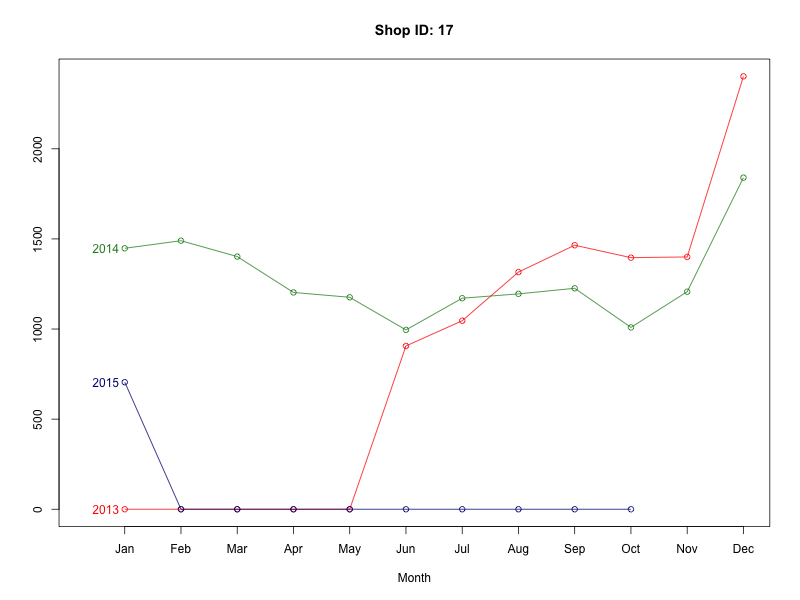
\includegraphics{../graphs/monthlyaverages_shop_id_17.png}
\caption{Monthly sales for Shop 17}
\end{figure}

\texttt{shop\_id} 38 shows a downward trend in sales year over year,
with seasonality showing sales spikes in March, August and December.

\begin{figure}
\centering
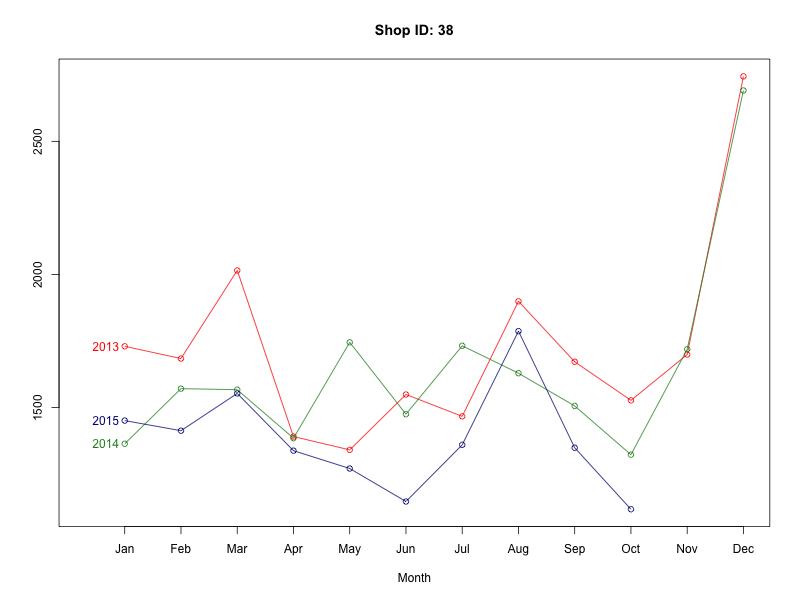
\includegraphics{../graphs/monthlyaverages_shop_id_38.png}
\caption{Monthly sales for Shop 38}
\end{figure}

\paragraph{Weekly Aggregations}\label{weekly-aggregations}

These were especially useful in time series clustering described in the
next section.

\subsubsection{Time Series Clustering}\label{time-series-clustering}

The \texttt{TSClust} package offers unsupervised clustering methods for
time series objects. While the package offers several dissimilarty
measures, after some investigation, the dissimilarity measure calcuated
using a Pearson's correlation coefficient between two time series seemed
to offer the best balance between simplicity, intuition, and
explanability of the results.

Hierarchical clustering is performed on the dissimilarity matrix on
weekly aggregated data using either the \emph{Complete Linkage} or the
\emph{Ward.D2} algorithm, depending which performs better by visual
inspection of the clusters. The results for three categorical variables
are shown below with details on how this insights affects subsequent
analyses.

\paragraph{Item Category - Level 1}\label{item-category---level-1}

The clusters highlighted in red boxes correspond to the color coding of
the time series plots. Right away, the power of this approach to isolate
or group signals together can be seen.

\begin{itemize}
\tightlist
\item
  \emph{Payment Cards} and \emph{Office} both have flatter beginnings
  with a bulge centering at week 110
\item
  \emph{Delivery of goods} and \emph{MAC Games} show spiky behaviour
\item
  \emph{Tickets}, \emph{Official} and \emph{PC} only had intermittent
  sales (possible sales-events), but are zero throughout
\item
  Many of the remainder of the signals (in yellow and gray) show
  trending and some seasonal behaviour
\end{itemize}

\begin{figure}
\centering
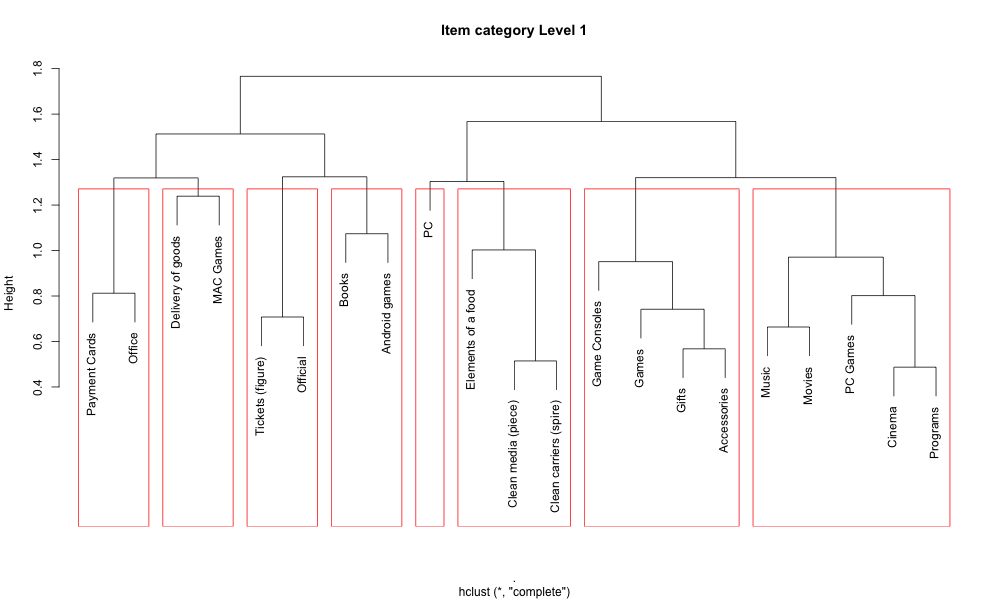
\includegraphics{../graphs/hclust_itemcat.png}
\caption{Hierarchical clustering dendogram for \texttt{itemcat\_lvl1}}
\end{figure}

\begin{figure}
\centering
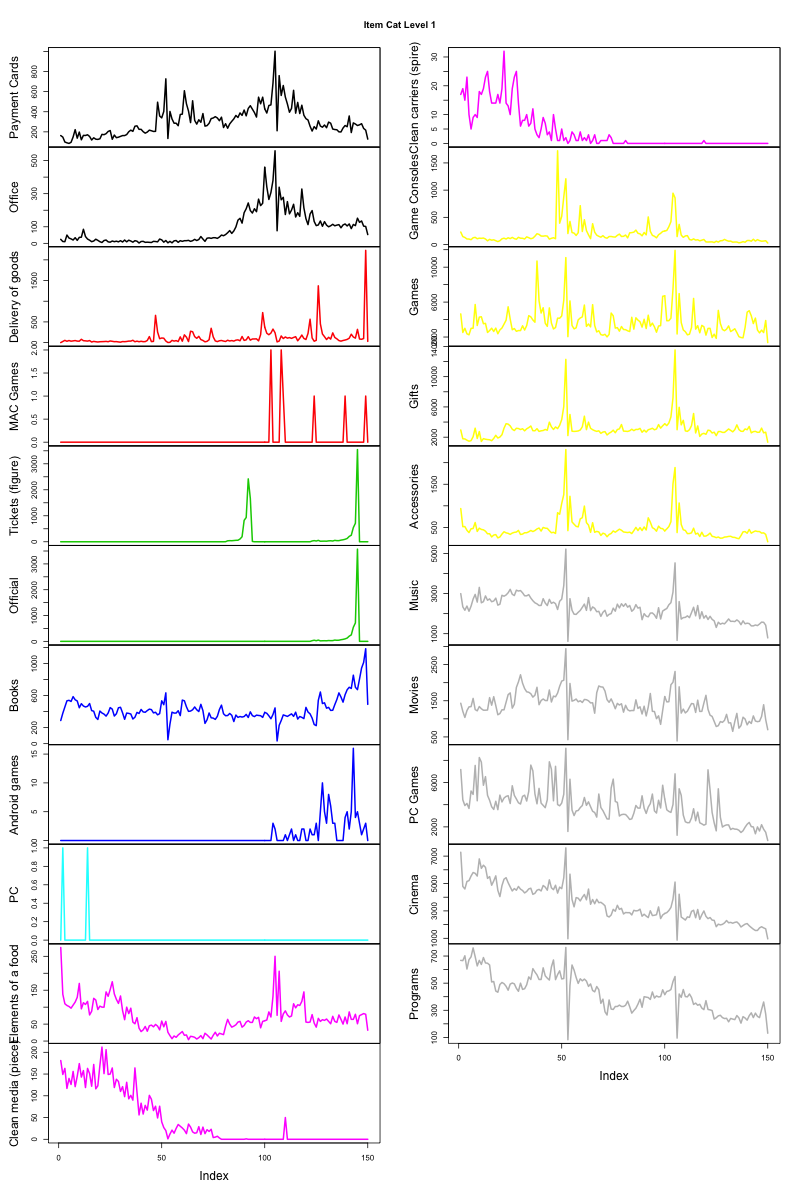
\includegraphics{../graphs/zoo_clust_itemcat.png}
\caption{Weekly aggregated time series for \texttt{itemcat\_lvl1}, color
coded by clusters identified using hierarchical clustering}
\end{figure}

\paragraph{Shop ID}\label{shop-id}

\texttt{shop\_id} shows five distinct groups of time series. Insights
gained from this analyis are:

\begin{itemize}
\tightlist
\item
  The black lines have a clear downward trend component
\item
  The red lines don't have much of a trend
\item
  Shop 36 has just opened up two months ago; not much data there
\item
  The blue lines start midway through the time series
\item
  The cyan lines are much spikier. The spiked identified by the red
  arrows line up with perfectly with those identified above for
  \emph{Delivery of goods}, \emph{Tickets} and \emph{Official} which
  helps treat these two shops with some special care before modeling
\end{itemize}

\begin{figure}
\centering
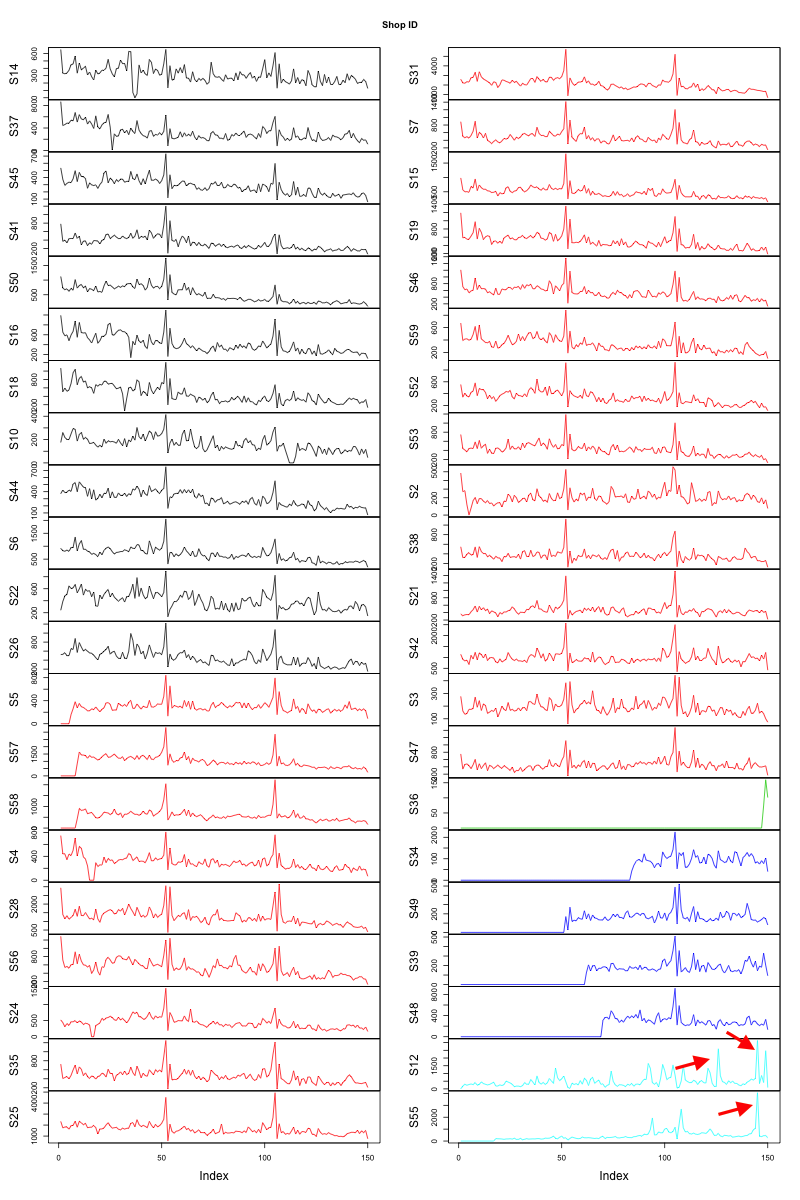
\includegraphics{../graphs/zoo_clust_shopid.png}
\caption{Weekly aggregated time series for \texttt{shop\_id}, color
coded by clusters identified using hierarchical clustering}
\end{figure}

\paragraph{Week Number}\label{week-number}

The week number clustering returns in very useful insights. Week 53 and
Week 1 - at the end and beginning of a year - had drastically different
sales patterns. Interestingly, Week 39 was the most different from the
rest, and could coincide with a russian holiday.

\begin{figure}
\centering
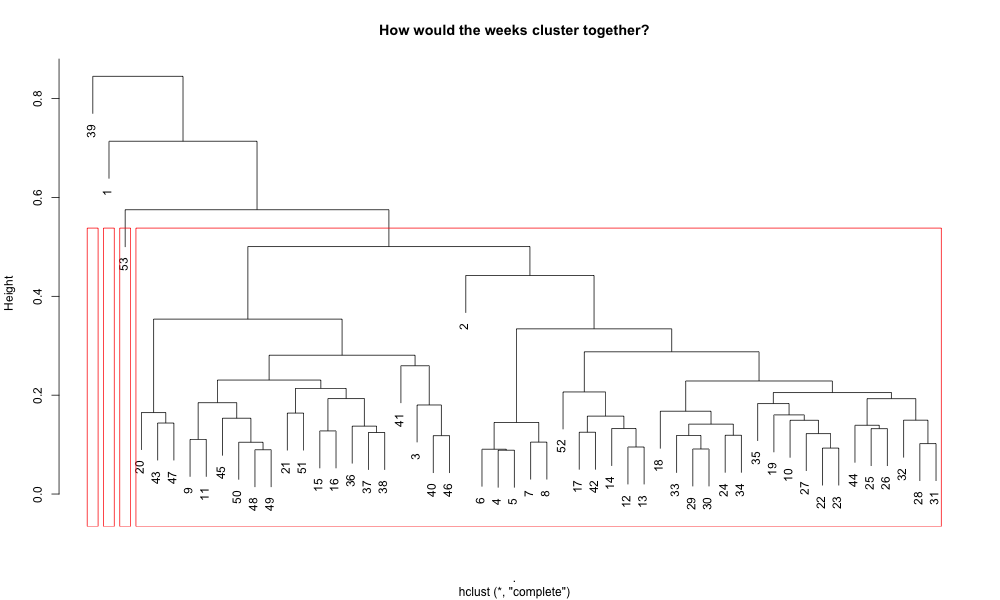
\includegraphics{../graphs/hclust_week.png}
\caption{Hierarchical clustering dendogram for \texttt{week\_number}}
\end{figure}

\subsection{Summary of Data Preparation
Activities}\label{summary-of-data-preparation-activities}

This is the summary of all the data preparation activities carried out:

\begin{itemize}
\tightlist
\item
  Data cleansing

  \begin{itemize}
  \tightlist
  \item
    Item categories \emph{Delivery of goods} is de-spiked
  \item
    Few negative values for \texttt{item\_cnt\_day} were replaced by
    positive values
  \item
    Text data is cleaned by removing trailing spaces, special
    characters, case correction and de-duplication
  \end{itemize}
\item
  Data removal

  \begin{itemize}
  \tightlist
  \item
    16 out of 60 shops had closed before Oct-2015 and are removed
  \item
    Item categories \emph{Tickets}, \emph{Official} are one-off sales
    and are removed
  \end{itemize}
\item
  Feature addition

  \begin{itemize}
  \tightlist
  \item
    In addition to the features described before, indicator variables
    for certain week numbers are added
  \end{itemize}
\end{itemize}

The resulting \texttt{master} data frame taken into analysis had
2,413,246 rows and 26 columns. Each analysis technique explored below
modified this data frame by aggregation and
addition/modification/removal of features.

\section{Modeling}\label{modeling}

The modeling approaches used for this project can be classified as a
\enquote{Top Down} approach. At a high level, this means:

\begin{enumerate}
\def\labelenumi{\arabic{enumi}.}
\tightlist
\item
  The Nov forecast for each shop (using \texttt{shop\_id}) is
  calculated. This may be either on daily, weekly or monthly aggregated
  data.
\item
  The next step is to calculate either the
  \texttt{level\ 1\ item\ category} or the \texttt{item\_id}, depending
  on the approach.
\end{enumerate}

A total of 8 models are built including one ensemble model. Each concept
tweaks both these steps slighly to build a diverse set of models. The
ensemble model is a simple average of the top 3 models.

\subsection{Overview of Approaches}\label{overview-of-approaches}

Here is an overview of the models executed for this project.

\begin{table}[H]

\caption{\label{tab:unnamed-chunk-5}Model Details}
\centering
\resizebox{\linewidth}{!}{\begin{tabular}[t]{lllll}
\toprule
Concept & Model Type & R Command & Aggregation & Comments\\
\midrule
C1 & Seasonal Naïve & forecast::snaive() & Monthly & \\
C2a & Time Series Linear Model & forecast::tslm() & Weekly & item\_id level models\\
C2b & Time Series Linear Model & forecast::tslm() & Monthly & item\_id level models\\
C3a & ARIMA & forecast::auto.arima() & Weekly & Top down approach\\
C3b & ARIMA & forecast::auto.arima() & Monthly & Top down approach\\
\addlinespace
C4 & Prophet & facebook::prophet() & Daily & Top down approach\\
C5 & TBATS & forecast::tbats() & Weekly & Top down approach\\
C6 & STLF with Auto-BoxCox & forecast::stlf() & Weekly & Top down approach\\
C7 & Ensemble &  &  & C3a+C4+C5\\
\bottomrule
\end{tabular}}
\end{table}

A discussion of some of the more interesting approaches follows.

\subsubsection{Concept 3a and 3b}\label{concept-3a-and-3b}

The approach described here in pseudocode roughly applies to concepts
C4, C5 and C6 as well. The top-down approach for this concept is as
follows:

\begin{itemize}
\tightlist
\item
  Clean and prep that data. Develop the matrix for \texttt{xreg} portion
  of \texttt{auto.arima()}
\item
  For each \texttt{shop\_id}, fit an \texttt{auto.arima} model with
  \texttt{seasonal\ =\ TRUE}. Forecast out 4 weeks or 1 month, depending
  on the concept. The 2015-Nov total sales forecast is now ready. (A)
\item
  For each \texttt{item\_id}, calculate the percent sales of that item
  per shop. (B)
\item
  Multiply (A) and (B) to estimate the \texttt{item\_id}'s sales volume
  for 2015-Nov. (C)
\item
  There will be still a large number of missing values. Here is how to
  tackle them.

  \begin{itemize}
  \tightlist
  \item
    Step 1 - Estimate the average item sales per month for each
    \texttt{item\_id}. {[}Essentially, a \texttt{meanf} model is
    used.{]}
  \item
    Step 2 - Aggregate this average for the year of 2015 and use this
    average for missing values in (C)
  \item
    Step 3 - For the remainder of missing values, set them to zero
  \item
    Step 4 - Clip the results between 0 and 20
  \end{itemize}
\end{itemize}

\subsubsection{Concept 4 - Prophet
Models}\label{concept-4---prophet-models}

Prophet is a package developed by Facebook for robust, scalable time
series forecasting. To quote the package authors, \enquote{Prophet is a
procedure for forecasting time series data. It is based on an additive
model where non-linear trends are fit with yearly and weekly
seasonality, plus holidays. It works best with daily periodicity data
with at least one year of historical data. Prophet is robust to missing
data, shifts in the trend, and large outliers}.

The advantage of this package is in it's robustness to outliers and it's
ability to handle low-count based data while still operating on
un-aggregated daily input data. It's fast and came up with reliable
forecasts. For this concept, 573 \texttt{shop\_id} +
\texttt{item\_category\_id} level models are built.

A few examples of these forecasts are shown in figures 7 and 8. Each
black point is a daily observation, while the blue lines are the
forecasts and prediction intervals.

\begin{figure}
\centering
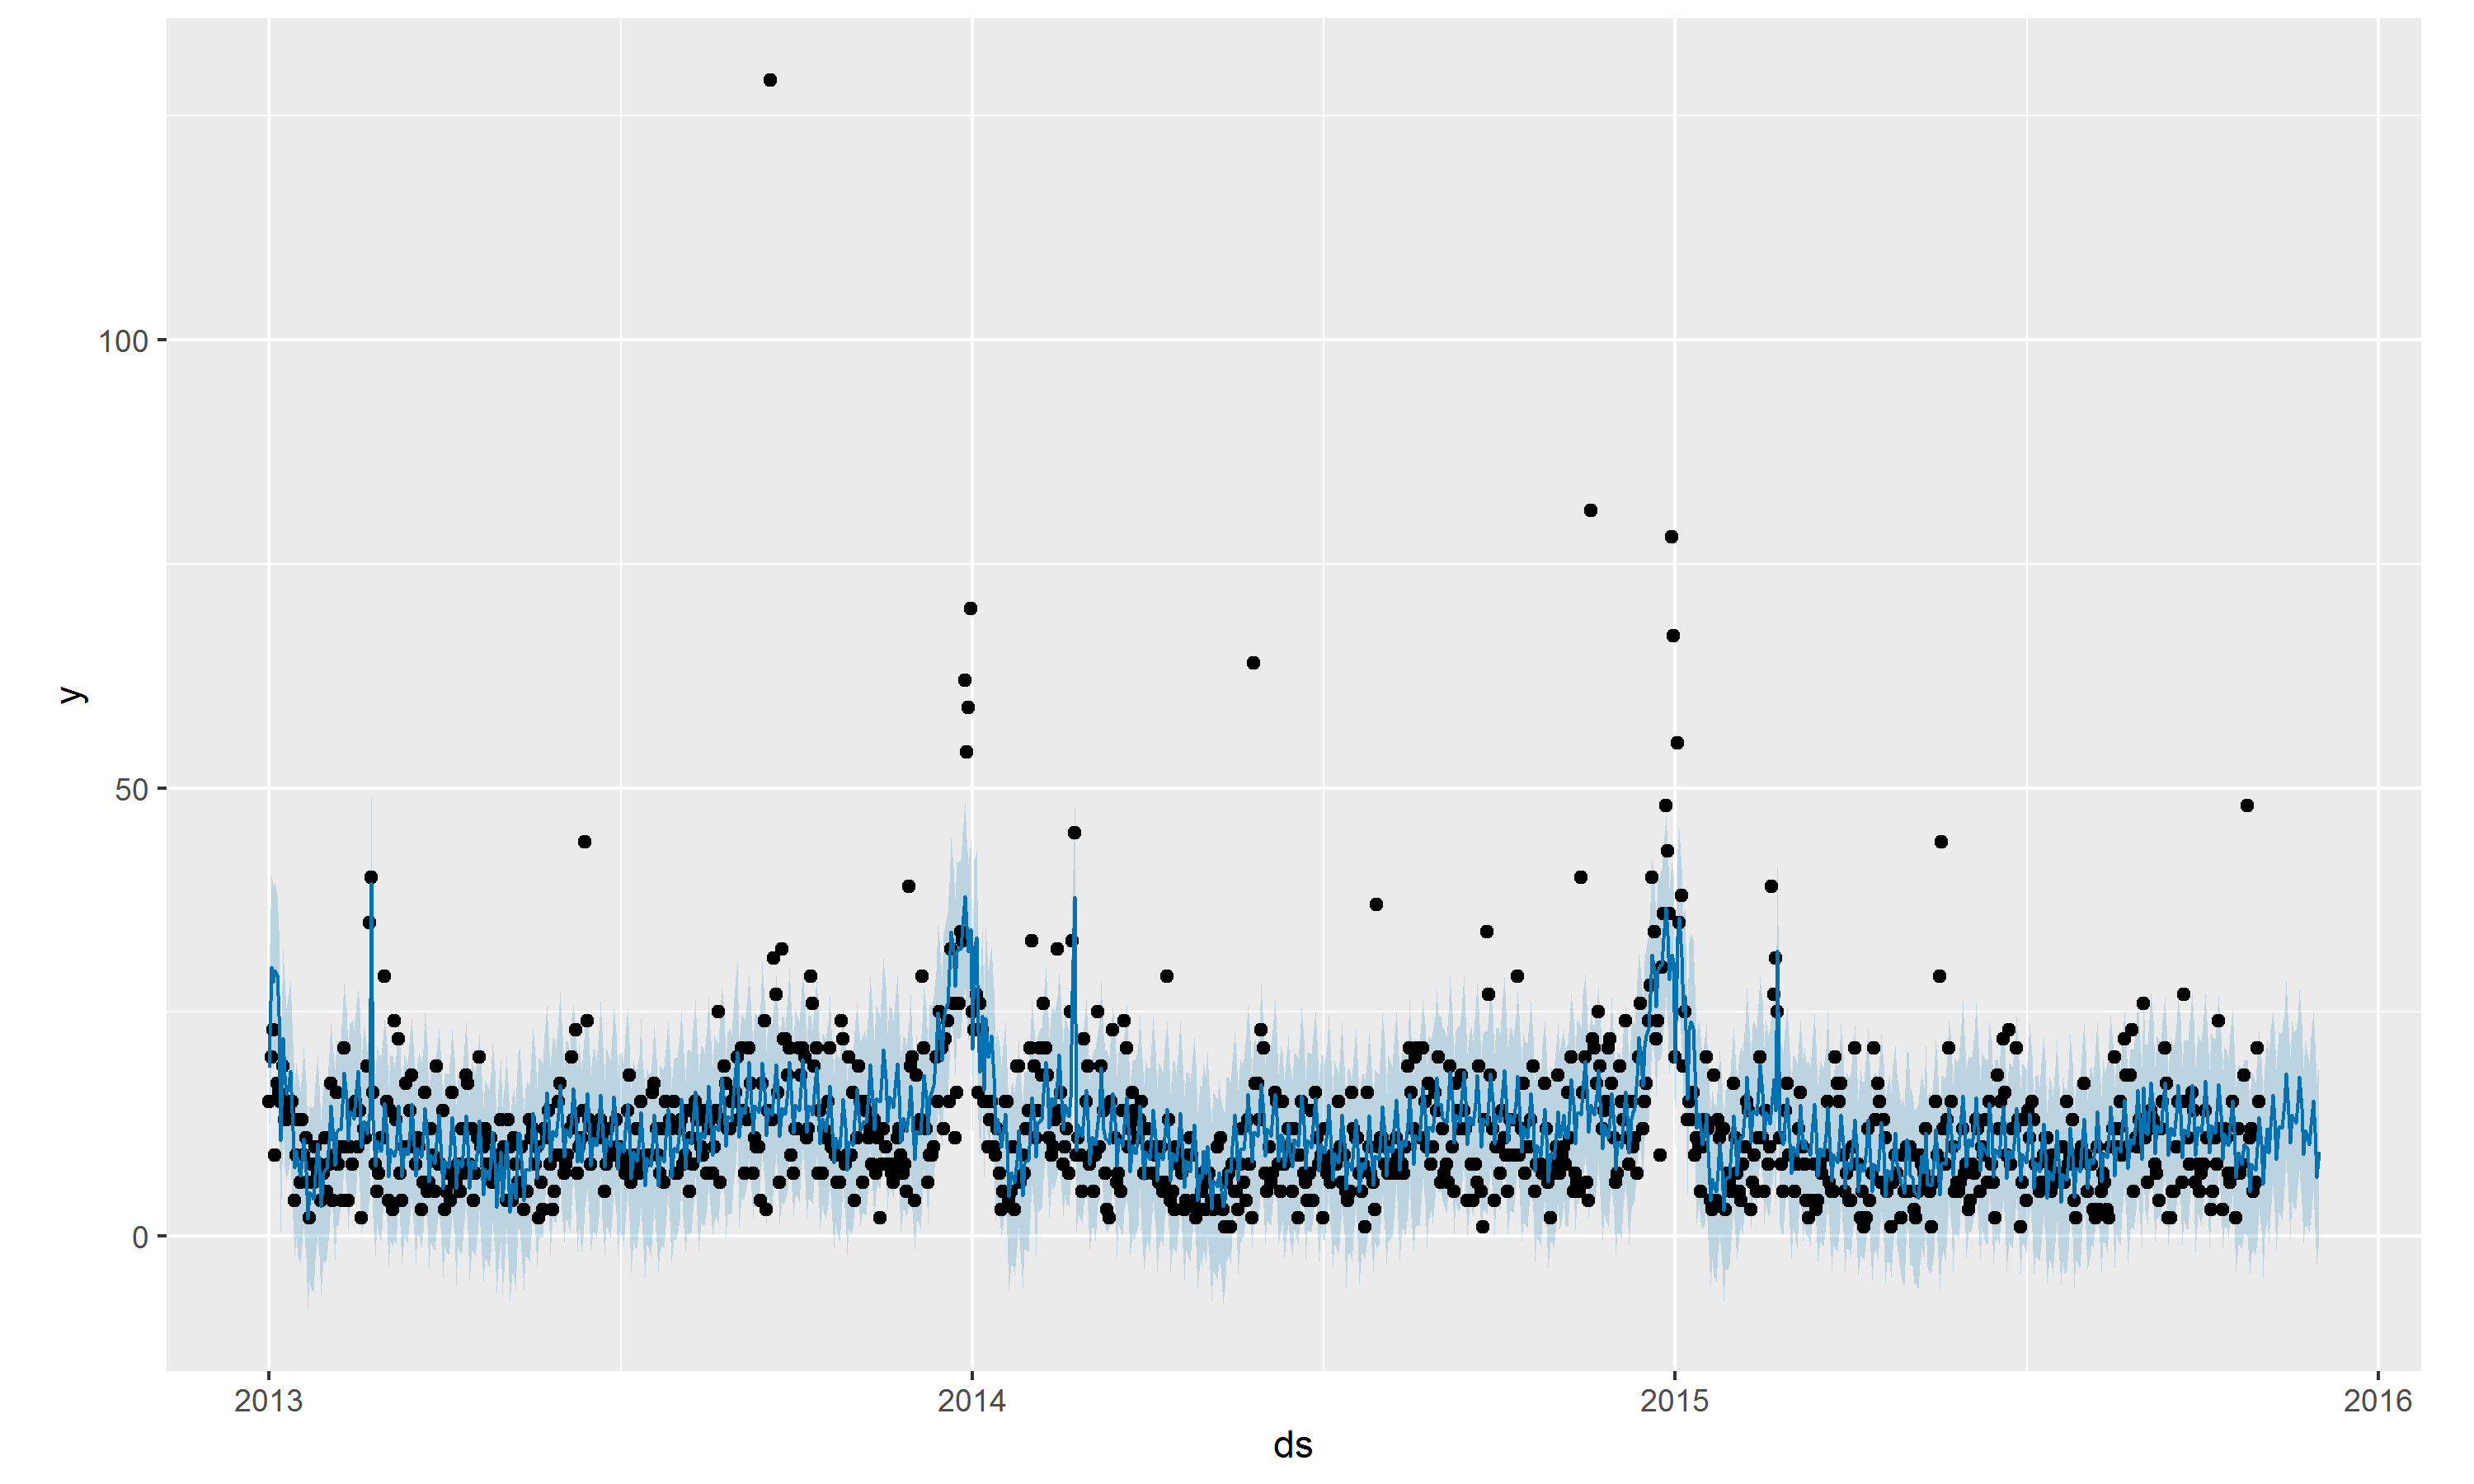
\includegraphics{../graphs/prophet/S15Games.png}
\caption{Shop 15 - Games}
\end{figure}

\begin{figure}
\centering
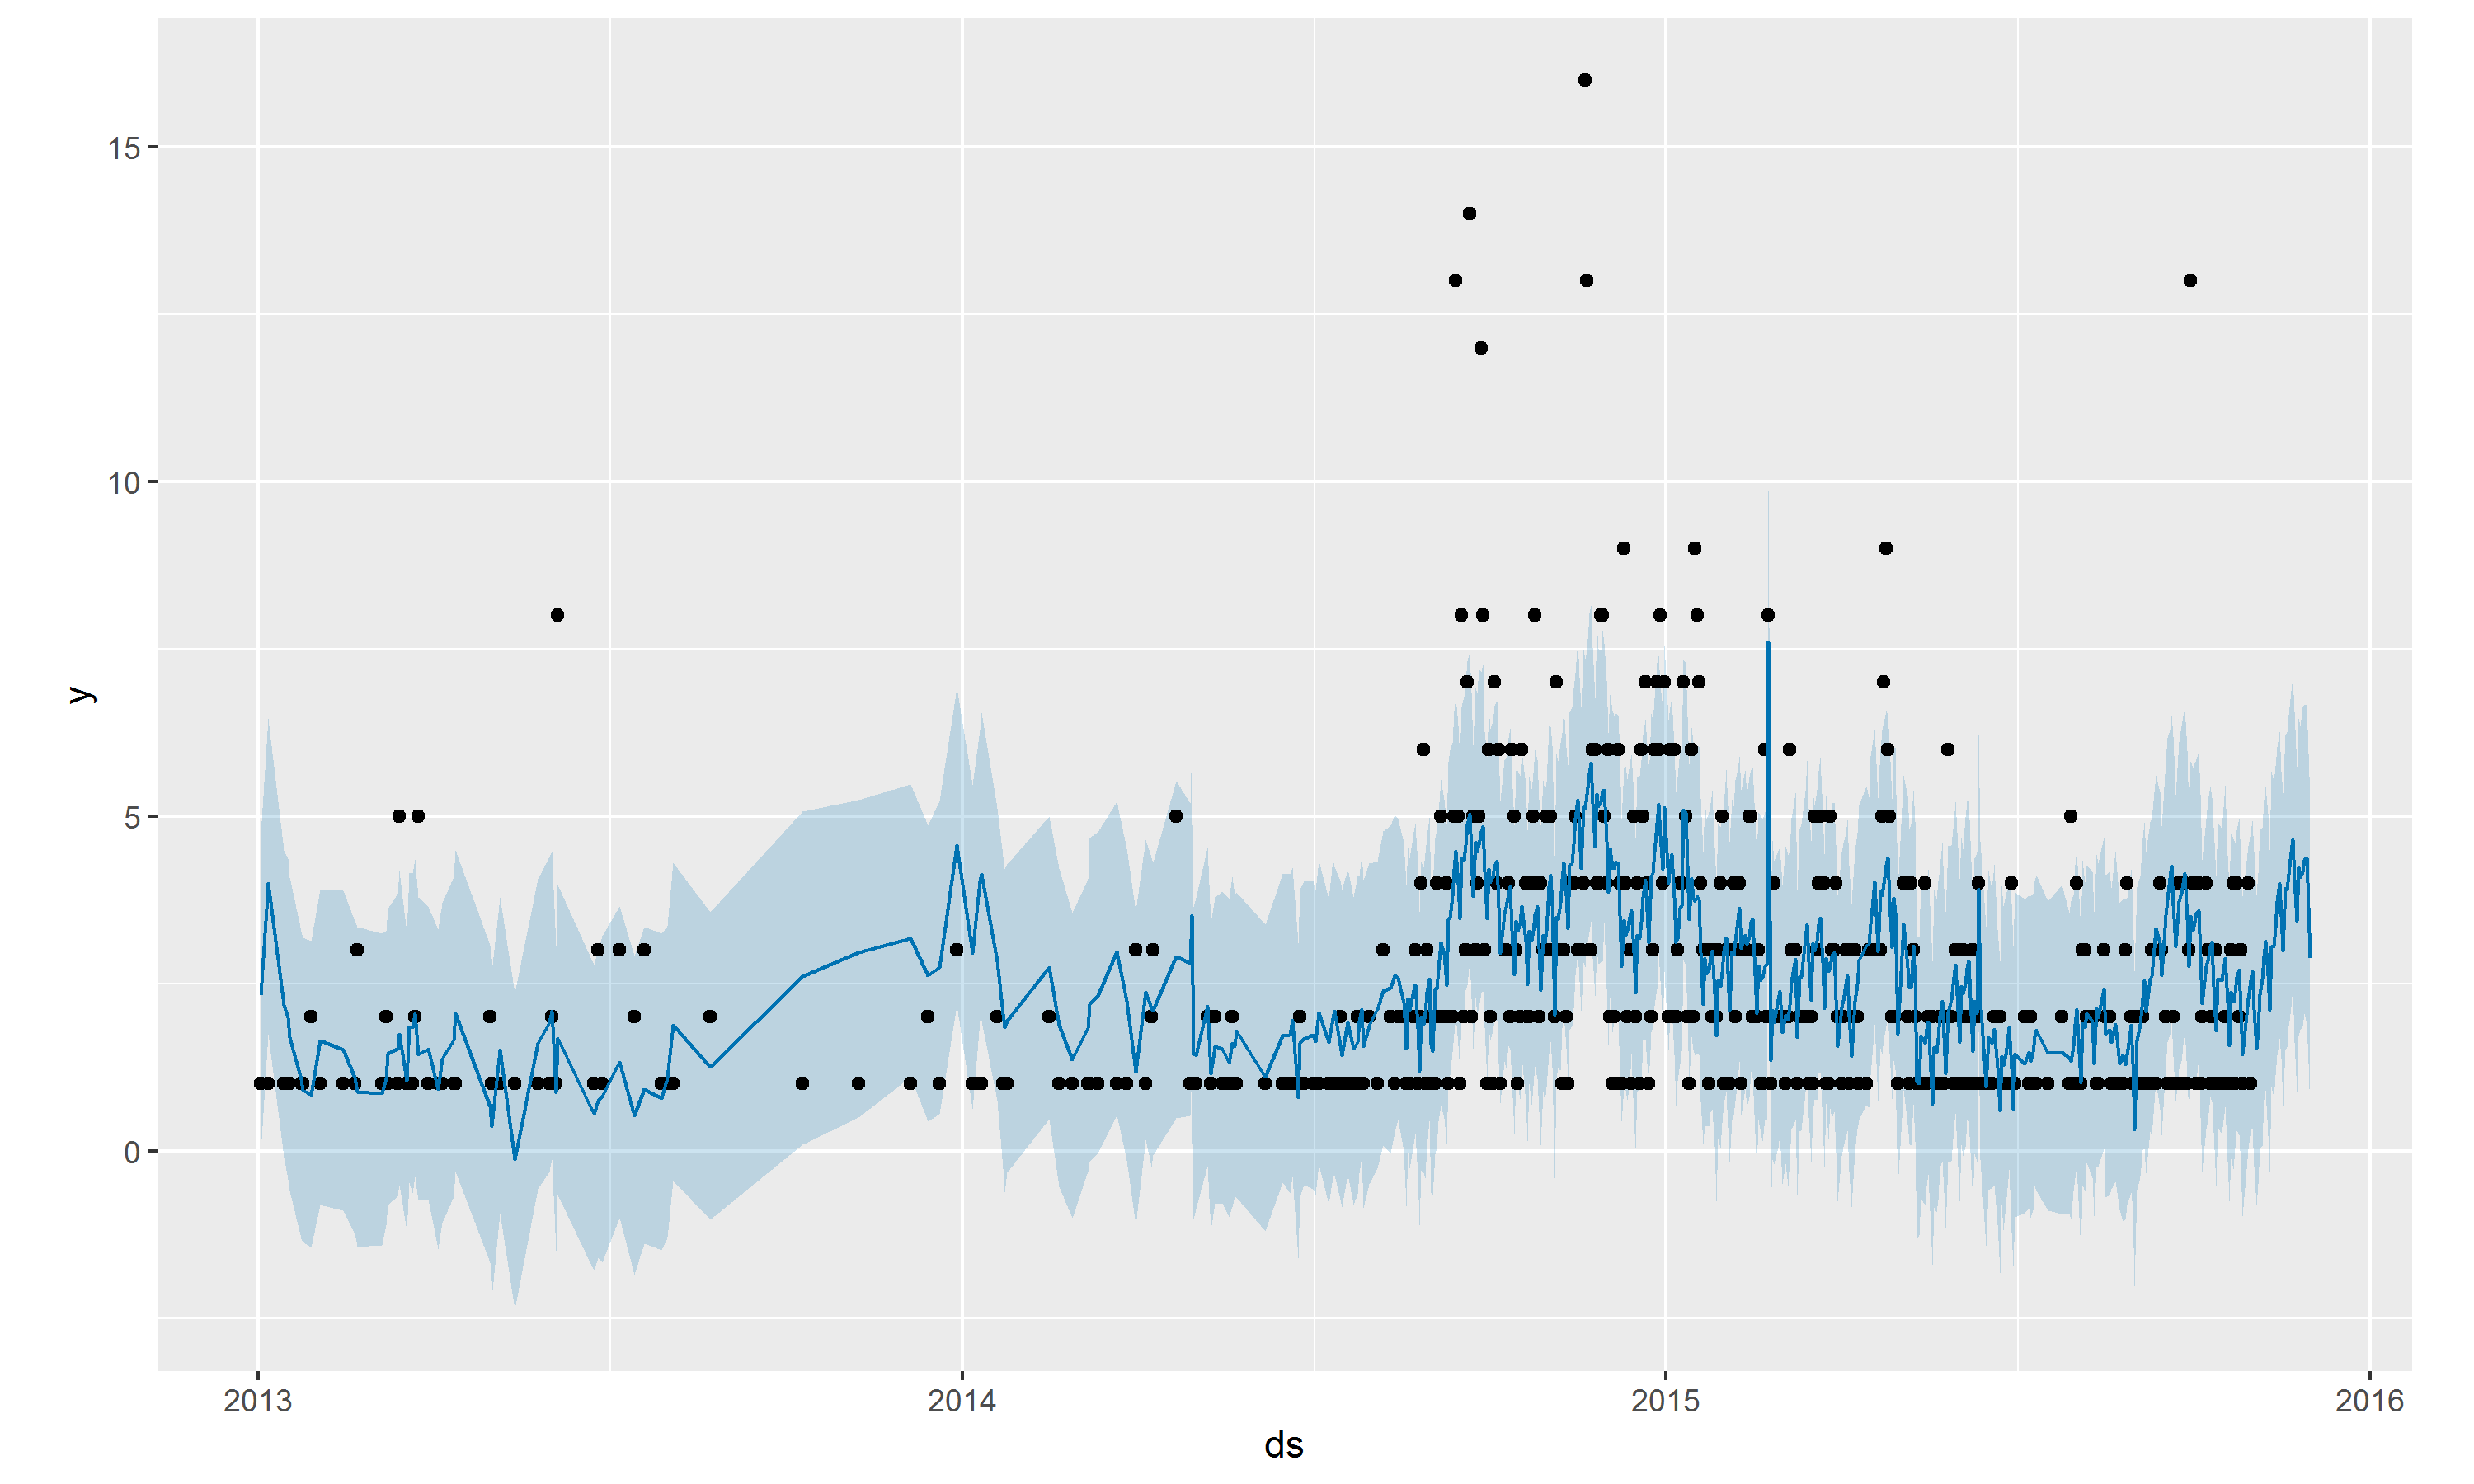
\includegraphics{../graphs/prophet/S31Office.png}
\caption{Handling low count data - Shop 31 - Office}
\end{figure}

\subsubsection{Concept 6}\label{concept-6}

\subsection{Programming Details}\label{programming-details}

Given the large number of models programmatically fit, as shown in the
table below, one of the challenges was to get these to run on a smaller
machine, using single core processing. The solution was to move to a
40-core 128GB machine and leverage a
\texttt{foreach(...)\ \%dopar\%\ \{...\}} approach using the
\texttt{doParallel} and \texttt{foreach} package. This brough the
computation time from \textasciitilde{}3-4 hours to
\textasciitilde{}5-15 minutes.

\begin{table}[H]

\caption{\label{tab:unnamed-chunk-6}Model Details}
\centering
\begin{tabular}[t]{lll}
\toprule
Concept & Model Type & No of Fits\\
\midrule
C1 & Seasonal Naïve & Nil\\
C2a & Time Series Linear Model & 337,084\\
C2b & Time Series Linear Model & 337,084\\
C3a & ARIMA & 42\\
C3b & ARIMA & 42\\
\addlinespace
C4 & Prophet & 573\\
C5 & TBATS & 573\\
C6 & STLF with Auto-BoxCox & 573\\
\bottomrule
\end{tabular}
\end{table}

\section{Results Summary}\label{results-summary}

Given the complexity of the code structure required to automate
execution and book-keeping of such a large set of models, it was not
feasible within the given time frame to book-keep, extract and inspect
the traditional metrics of AICc, BIC, RMSE or MASE from each of the
\texttt{forecast} objects. The models were evaluated based on their test
set Kaggle scores. The Kaggle scores themselves represent
\textasciitilde{}25\% of the test data, but give a decent indication of
model performance.

\begin{table}[H]

\caption{\label{tab:unnamed-chunk-7}Model Details}
\centering
\begin{tabular}[t]{lllr}
\toprule
Concept & Model Type & Aggregation & Kaggle Score\\
\midrule
C1 & Seasonal Naïve & Monthly & 3.77\\
C2a & Time Series Linear Model & Weekly & 3.94\\
C2b & Time Series Linear Model & Monthly & 4.03\\
C3a & ARIMA & Weekly & 1.21\\
C3b & ARIMA & Monthly & 4.04\\
\addlinespace
C4 & Prophet & Daily & 1.38\\
C5 & TBATS & Weekly & 1.24\\
C6 & STLF with Auto-BoxCox & Weekly & 1.25\\
C7 & Ensemble & Weekly & 1.24\\
\bottomrule
\end{tabular}
\end{table}

\begin{figure}
\centering
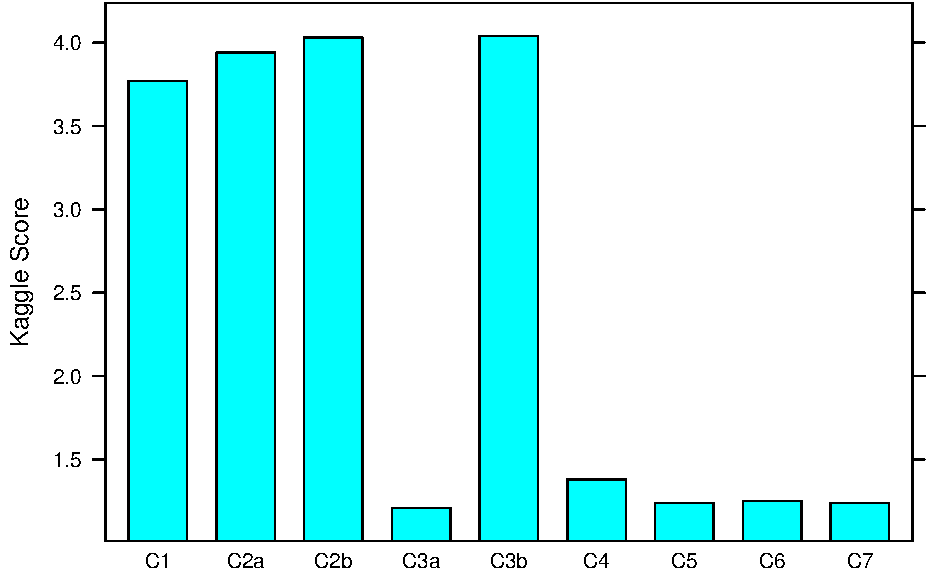
\includegraphics{Final_report_files/figure-latex/unnamed-chunk-8-1.pdf}
\caption{}
\end{figure}

The final two models selected for Kaggle submission are C3a (Weekly
aggregated Auto ARIMA) and C7 (Ensemble model of C3a, C4 and C5).

\section{Limitations}\label{limitations}

As can be seen from the Kaggle scores, the top-down approach seems to
have stabilized at a score of \textasciitilde{}1.2, irrespective of the
underlying model used - ARIMA, TBATS or STLF for weekly aggregation, or
Prophet for daily aggregation. The bottleneck in this approach is surely
the subsequent steps of estimation of the the \texttt{item\_id}
forecasts using simple non-trending proportions calculated over the 2015
data. Even upon further parameter tuning (BoxCox transformations,
outlier/spike removals, different methods of handling NA values,
addition/removal of regressors from \texttt{xreg} in
\texttt{auto.arima()}, different holiday dates etc), the lowest Kaggle
score achieved could not be beat, which points to a plateau being hit
for this top-down forecasting approach. To improve this score further,
some major change needs to occur - either in the preprocessing, or model
strategy.

\section{Future work}\label{future-work}

These are ideas yet to be explored for this challenge:

\begin{itemize}
\tightlist
\item
  Utilization of 2-layered models where the residuals of one feed into
  the next model
\item
  Utilization of logistic regression based approaches
\item
  Further hyper parameter tuning of the \texttt{Prophet} package calls
\item
  Utilization of machine learning approaches like \texttt{xgboost} or
  \texttt{LSTM}
\item
  SVD based approaches are documented to be successful here:
  \url{https://www.kaggle.com/c/walmart-recruiting-store-sales-forecasting/discussion/8125}
\end{itemize}

\section{Challenges and learnings}\label{challenges-and-learnings}

Apart from the computational challenges addressed via parallel
computation listed above, the other computational challenge faced was
when an xgboost model was attempted at an \texttt{item\_id} level. Since
xgboost can only handle numerical variables, transformation of 8000+
levels to an extremely sparse dummy-matrix (required 308 GB RAM to
perform) was not possible. Either this is a computational challenge, or
a conceptual weakness on how to correctly use xgboost on my part.

Secondly, all the EDA, plotting and clustering really highlighted the
importance of exploration at the front end of any analyses. It also
helps tremenously to be strong at a language like R to be able to
automate many of these tasks.

\newpage

\section{R Packages Used}\label{r-packages-used}

\begin{itemize}
\tightlist
\item
  remedy\_0.0.0.9600\\
\item
  bindrcpp\_0.2.2\\
\item
  prophet\_0.2.1
\item
  Rcpp\_0.12.16\\
\item
  doParallel\_1.0.11\\
\item
  iterators\_1.0.9
\item
  foreach\_1.4.4
\item
  plotly\_4.7.1\\
\item
  zoo\_1.8-1\\
\item
  magrittr\_1.5
\item
  Rtsne\_0.13
\item
  timeDate\_3043.102\\
\item
  xgboost\_0.6.4.1
\item
  caret\_6.0-79
\item
  TSclust\_1.2.4
\item
  cluster\_2.0.7-1\\
\item
  pdc\_1.0.3\\
\item
  wmtsa\_2.0-3
\item
  janitor\_1.0.0\\
\item
  sweep\_0.2.1
\item
  forecast\_8.3
\item
  lattice\_0.20-35
\item
  lubridate\_1.7.4
\item
  plyr\_1.8.4\\
\item
  reshape2\_1.4.3\\
\item
  ProjectTemplate\_0.8.2
\item
  kableExtra\_0.8.0
\item
  knitr\_1.20\\
\item
  forcats\_0.3.0
\item
  stringr\_1.3.0
\item
  dplyr\_0.7.4
\item
  purrr\_0.2.4\\
\item
  readr\_1.1.1\\
\item
  tidyr\_0.8.0
\item
  tibble\_1.4.2
\item
  ggplot2\_2.2.1\\
\item
  tidyverse\_1.2.1
\item
  papaja\_0.1.0.9709
\end{itemize}

\newpage

\section{References}\label{references}

\begin{itemize}
\tightlist
\item
  \url{https://www.jstatsoft.org/article/view/v062i01/v62i01.pdf}
\item
  \url{https://peerj.com/preprints/3190.pdf}
\item
  \url{https://facebook.github.io/prophet/}
\item
  \url{https://www.kaggle.com/c/walmart-recruiting-store-sales-forecasting/discussion/8125}
\item
  \url{https://www.kaggle.com/c/walmart-recruiting-store-sales-forecasting/discussion/8033}
\end{itemize}

\begingroup
\setlength{\parindent}{-0.5in} \setlength{\leftskip}{0.5in}

\hypertarget{refs}{}

\endgroup






\end{document}
